% PAKETE UND DOKUMENTKONFIGURATION
\documentclass[11pt, a4paper]{article}

% Encoding für Umlaute
\usepackage[utf8]{inputenc}
\usepackage[T1]{fontenc}

% Silbentrennung
\usepackage[ngerman]{babel}

% erweiterte Matheumgebungen und Formelnummer mit Sectionnummer
\usepackage{amsmath}
\numberwithin{equation}{section}

% Braket Notation
\usepackage{braket}

% zusätzliche mathematische Schriftarten
\usepackage{amsfonts}

% verschiedene mathematische Symbole
\usepackage{amssymb}

% Einheiten setzen z.B. \SI{10}{\kilo\gram\meter\per\second\squared}
% Fehler: \SI{10 +- 0,2e-4}{\metre}
\usepackage{siunitx}
\sisetup{
  output-decimal-marker={,},
  separate-uncertainty
}

% Randbreiten
\usepackage[left=3.5cm,right=3.5cm,top=3cm,bottom=3cm,twoside]{geometry}

% Bilder einfügen
\usepackage{graphicx}

% Verweise innerhalb des Dokuments
\usepackage{hyperref}
\hypersetup{
	colorlinks = true,
	allcolors = {black}
}

% bessere Tabellenlayouts
\usepackage{booktabs}
\usepackage{multirow}

% Seitenlayout (Kopfzeile)
\usepackage{fancyhdr}

% Float Barriers
\usepackage{placeins}

% Pakete für gedrehte Subfigures
\usepackage{caption}
\usepackage{subcaption}
\usepackage{rotating}

% Caption-Setup
\captionsetup{font={small}}
\renewcommand{\thefigure}{\thesection.\arabic{figure}}
\renewcommand{\thesubfigure}{\alph{subfigure}}
\renewcommand{\thetable}{\thesection.\arabic{table}}
\renewcommand{\thesubtable}{\alph{subtable}}

% Manuelle Silbentrennung
\hyphenation{}

% Tiefe des Inhaltsverzeichnisses (Level: 1 sections, 2 subsections,
% 3 subsubsections)
\setcounter{tocdepth}{3}

% FANCYHDR SETUP
\pagestyle{fancy}
\fancyhead[EL,OR]{\thepage}
\fancyhead[ER]{\leftmark}
\fancyhead[OL]{\rightmark}

\renewcommand{\sectionmark}[1]{
\markboth{\thesection{} #1}{\thesection{} #1}
}
\renewcommand{\subsectionmark}[1]{
\markright{\thesubsection{} #1}
}

% DOKUMENTINFORMATIONEN
\title{P442 \\ Laser}

\author{Christopher Deutsch\footnote{christopher.deutsch@uni-bonn.de} \and Christian Bespin\footnote{christian.bespin@uni-bonn.de}}

\date{\today}

\begin{document}

\begin{titlepage}

\maketitle

% DURCHFÜHRUNGSDATUM UND TUTOR
\begin{center}
\begin{tabular}{l r}
Durchführung: & 15./16. Dezember 2014 \\
Gruppe: & $\alpha$ 2 \\
Tutor: & Tobias Macha
\end{tabular}
\end{center}

% ZUSAMMENFASSUNG
\begin{abstract}
\noindent

\end{abstract}

\end{titlepage}

% INHALTSVERZEICHNIS
\tableofcontents
% Neue Seite nach TOC
\newpage

% INHALT VERSUCHSPROTOKOLL

\section{Einführung}

\section{Theorie}

\section{Durchführung und Auswertung}
Sofern nicht anders angegeben Durchführung wie in Praktikumsanleitung.

\subsection{Aufbau des Helium-Neon Experimentierlasers und Charakterisierung der Intensität}

\subsection{Bestimmung der Wellenlänge des Lasers mit einem Reflexionsgitter}
\subsubsection{Durchführung}
\begin{figure}[h]
	\centering
	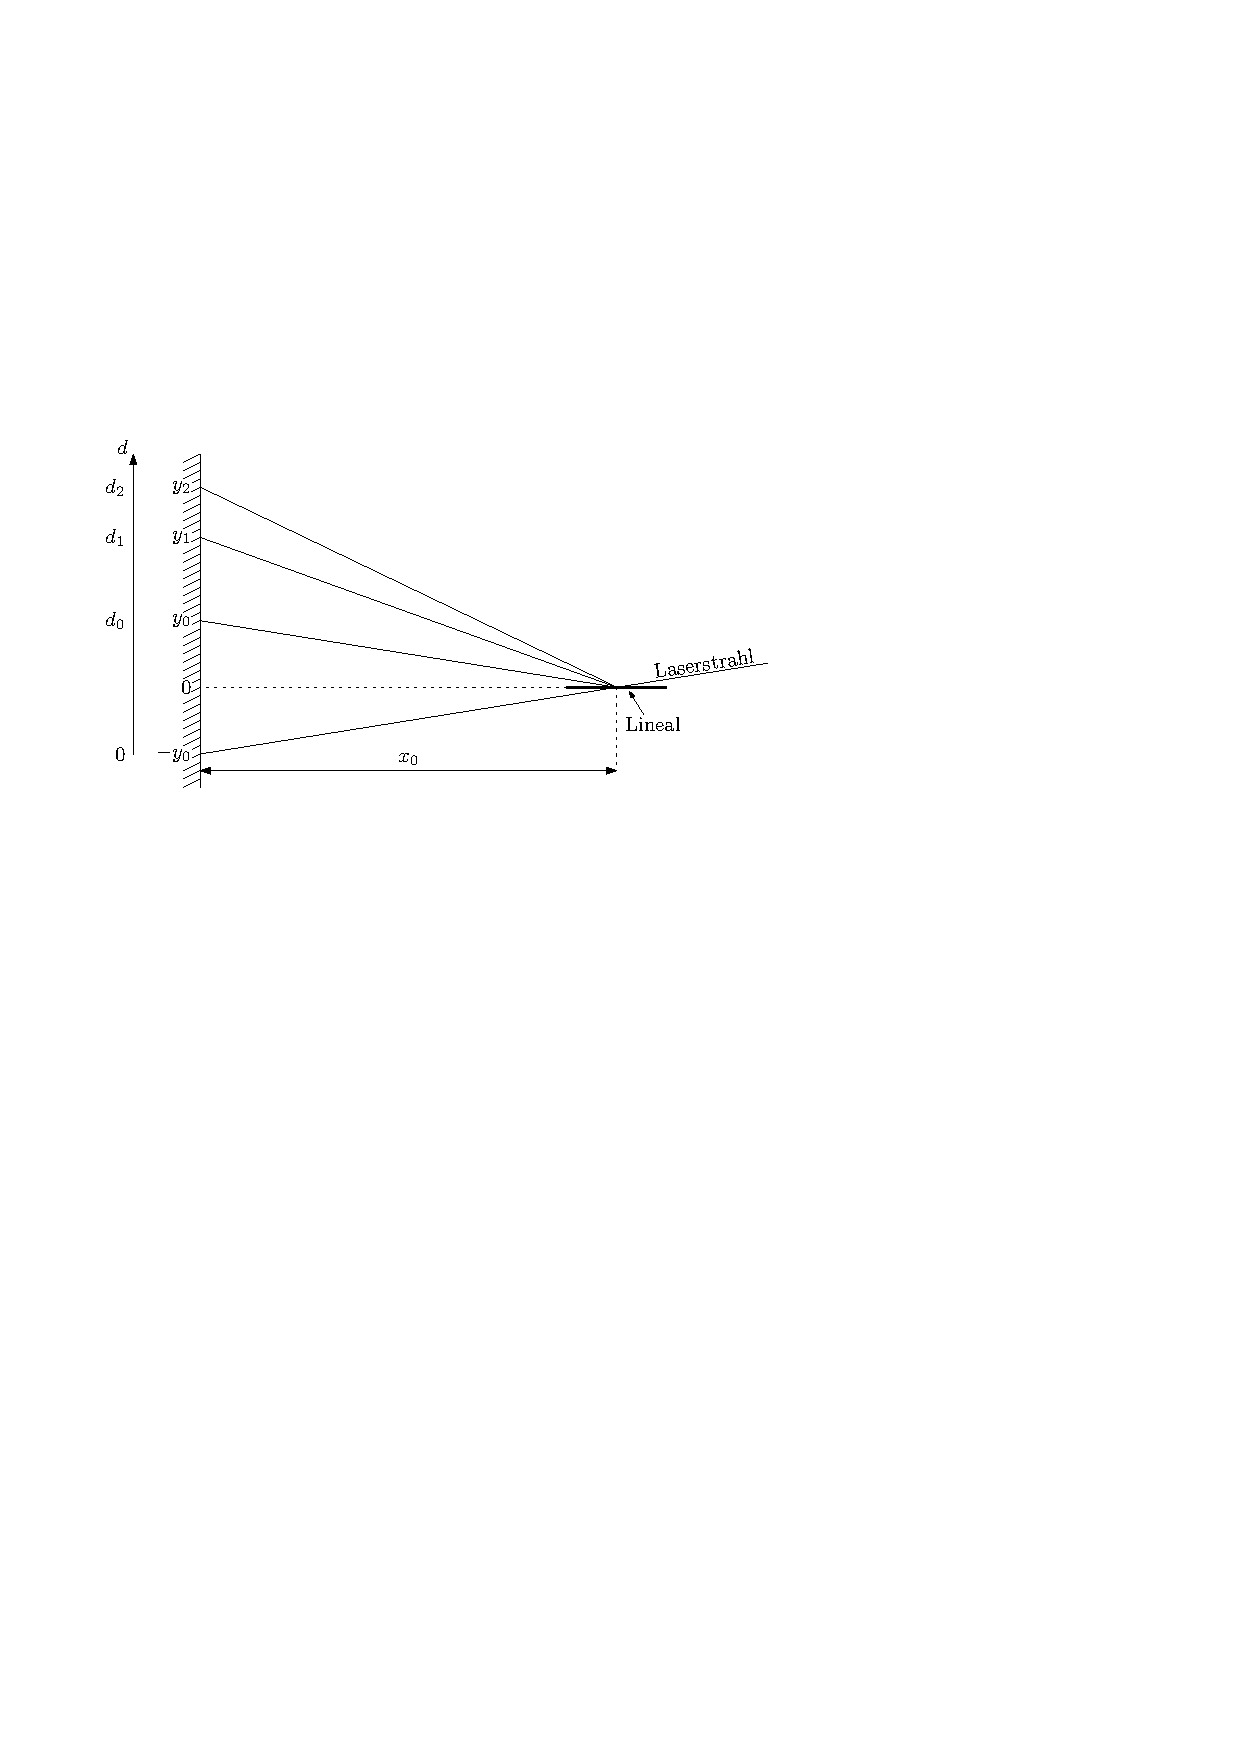
\includegraphics[width=0.9\textwidth]{./figures/wellenlaenge_lineal.pdf}
	\caption{Wellenlängenbestimmung nach Schawlow \cite{schawlow} und die im Versuch gemessenen Längen $d$}
	\label{fig:schawlow}
\end{figure}
Zur Bestimmung der Wellenlänge des Helium-Neon Lasers nach Schawlow \cite{schawlow} wird ein Stahlmaßstab mit eingravierter Skaleneinteilung als Reflexionsgitter verwendet.
Dazu wird der Laserstrahl in flachem Winkel auf die Millimeter-Skala des Maßstabes geleitet, sodass ein scharfes Interferenzmuster auf dem Whiteboard in einer Entfernung (von der Mitte der beleuchteten Stelle am Lineal) von $x_0 = \SI{252 +- 2}{\centi\metre}$ entsteht.
Anschließend werden die Maxima des Musters markiert, wobei darauf geachtet werden muss, dass bei der nullten Beugungsordnung begonnen wird, um negative Beugungsordnungen zu vermeiden.
Die nullte Beugungsordnung kann daran erkannt werden, dass sie maximale Intensität aufweist.
Nachdem ausreichend viele Ordnungen markiert wurden, wird das Lineal aus dem Strahlengang entfernt und der Auftreffpunkt des Laserstrahls auf dem Whiteboard markiert.
Schließlich wird mit einem Maßband die Position $d$ aller Beugungsmaxima relativ zum Auftreffpunkt des Lasers ohne Lineal gemessen (vergleiche dazu auch Abbildung \ref{fig:schawlow}).
Die Schärfe des Interferenzmusters ließ es dabei zu, die Längen $d$ mit einem abgeschätzten Fehler von $\Delta d = \SI{0.2}{\centi\metre}$ zu bestimmen.

\subsubsection{Auswertung}
In \cite{schawlow} wird gezeigt, dass für die Gittergleichung in Kleinwinkelnäherung ($\frac{y_n}{x_0} \ll 1$) gegeben ist:
\begin{align}
	n \lambda = \frac{1}{2} g \left( \frac{y_n^2 - y_0^2}{x_0^2} \right) \text{,}
	\label{eq:gittergleichung_schawlow}
\end{align}
wobei $g$ die Gitterkonstante ist und ansonsten die Notation aus Abbildung \ref{fig:schawlow} verwendet wird.
Um aus den gemessenen Werten $d_n$ die Wellenlänge zu bestimmen, muss zunächst die Position $y_0$ des reflektierten Strahls auf dem Schirm berechnet werden, welche gemäß Abbildung \ref{fig:schawlow} gegeben ist durch:
\begin{align}
	y_0 = \frac{d_0}{2} \text{,}
\end{align}
sodass mit dem gemessenen Wert $d_0 = \SI{19.7 +- 0.2}{\centi\metre}$ folgt:
\begin{align}
	y_0 = \SI{9.85 +- 0.10}{\centi\metre} \text{.}
\end{align}
So kann die Position $y_n$ des $n$-ten Interferenzmaximums berechnet werden durch:
\begin{align}
	y_n &= d_n - y_0 \\
	\Delta y_n &= \sqrt{\Delta d_n^2 + \Delta y_0^2}
\end{align}
und anschließend mit der genäherten Gittergleichung \ref{eq:gittergleichung_schawlow} die Wellenlänge des Lasers für die einzelnen Maxima berechnet werden, wobei für die Gitterkonstante $g = \SI{1}{\milli\metre}$ gilt, da die Beugung an der Millimeter-Skala des Maßstabes stattfindet. 
Der Fehler der berechneten Wellenlänge $\Delta \lambda$ ist gegeben durch Gauß'sche Fehlerfortpflanzung unter der Vernachlässigung des Fehlers in der Gitterkonstanten $g$:
\begin{align}
	\Delta \lambda = \frac{g}{2 n} \sqrt{\left( \frac{2 y_n}{x_0^2} \right)^2 \cdot \Delta y_n^2 + \left( \frac{2 y_0}{x_0^2} \right)^2 \cdot \Delta y_0^2 + \left(\frac{2\left(y_n^2 - y_0^2 \right)}{x_0^3}\right)^2 \cdot \Delta x_0^2} \text{.}
\end{align}
Die gemessenen Abstände $d$ sowie die berechneten Werte wurden in Tabelle \ref{tab:wellenlaengen_berechnung} aufgetragen.
\begin{table}[h]
	\centering
	\begin{tabular}{SSSSSSS}
\toprule
{$n$} & {$d_n$ / \si{\centi\metre}} & {$\Delta d_n$ / \si{\centi\metre}} & {$y_n$ / \si{\centi\metre}} & {$\Delta y_n$ / \si{\centi\metre}} & {$\lambda$ / \si{\nano\metre}} & {$\Delta \lambda$ / \si{\nano\metre}} \\
\midrule
1  & 23.2 & 0.2 & 13.35 & 0.23 & 639 & 51 \\
2  & 26.0 & 0.2 & 16.15 & 0.23 & 645 & 32 \\
3  & 28.1 & 0.2 & 18.25 & 0.23 & 619 & 25 \\
4  & 30.2 & 0.2 & 20.35 & 0.23 & 624 & 21 \\
5  & 32.0 & 0.2 & 22.15 & 0.23 & 620 & 19 \\
6  & 34.0 & 0.2 & 24.15 & 0.23 & 638 & 18 \\
7  & 35.4 & 0.2 & 25.55 & 0.23 & 625 & 17 \\
8  & 37.1 & 0.2 & 27.25 & 0.23 & 635 & 16 \\
9  & 38.5 & 0.2 & 28.65 & 0.23 & 633 & 16 \\
10 & 39.7 & 0.2 & 29.85 & 0.23 & 625 & 15 \\
11 & 41.3 & 0.2 & 31.45 & 0.23 & 639 & 15 \\
12 & 42.4 & 0.2 & 32.55 & 0.23 & 632 & 14 \\
13 & 43.5 & 0.2 & 33.65 & 0.23 & 627 & 14 \\
14 & 44.8 & 0.2 & 34.95 & 0.23 & 632 & 14 \\
15 & 46.0 & 0.2 & 36.15 & 0.23 & 635 & 14 \\
16 & 47.1 & 0.2 & 37.25 & 0.23 & 635 & 14 \\
17 & 47.9 & 0.2 & 38.05 & 0.23 & 626 & 13 \\
18 & 49.2 & 0.2 & 39.35 & 0.23 & 635 & 13 \\
19 & 50.4 & 0.2 & 40.55 & 0.23 & 641 & 13 \\
\bottomrule
\end{tabular}
	\caption{Messdaten und Berechnung zur Wellenlängenbestimmung}
	\label{tab:wellenlaengen_berechnung}
\end{table}
Um aus den berechneten Wellenlängen für die einzelnen Maxima eine Wellenlänge zu bestimmen, wird der varianzgewichtete Mittelwert:
\begin{align}
	\bar{\lambda} = \frac{\sum_i \frac{\lambda_i}{\Delta \lambda_i^2}}{\sum_i \frac{1}{\Delta \lambda_i^2}}
\end{align}
verwendet, wobei dessen Fehler gegeben ist durch:
\begin{align}
\Delta \bar{\lambda} = \frac{1}{\sqrt{\sum_i \frac{1}{\Delta \lambda_i^2}}} \text{.}
\end{align}
Mit den Werten aus Tabelle \ref{tab:wellenlaengen_berechnung} folgt für die varianzgewichtete mittlere Wellenlänge:
\begin{align}
	\bar{\lambda} = \SI{632.0 +- 3.6}{\nano\metre} \text{.}
\end{align}
Der Vergleich mit dem Literaturwert \cite{NISTSpectra} für den ($\mathrm{5s} \rightarrow \mathrm{3p}$)-Übergang von Neon:
\begin{align}
	\lambda = \SI{632.81646}{\nano\metre}
\end{align}
liefert eine gute Übereinstimmung innerhalb des statistischen Fehlers.

\subsubsection{Vergleich mit der exakten Rechnung}
Schließlich soll die Verwendung der Näherungsformel gerechtfertigt werden.
Mit der Gittergleichung
\begin{align}
	n \lambda = g \left( \cos(\alpha) - \cos(\beta_n) \right)
	\label{eq:wellenlaenge_exakt}
\end{align}
und
\begin{align}
	\cos(\alpha) &= \frac{x_0}{\sqrt{x_0^2 + y_0^2}} \\
	\cos(\beta_n) &= \frac{x_0}{\sqrt{x_0^2 + y_n^2}}
\end{align}
folgt die relative Abweichung durch Quotientenbildung von Gleichungen \ref{eq:gittergleichung_schawlow} und \ref{eq:wellenlaenge_exakt}:
\begin{align}
	\frac{\Delta \lambda}{\lambda} = \frac{\lambda_\mathrm{KWN} - \lambda}{\lambda} = \frac{1}{2} \frac{\frac{y_n^2 - y_0^2}{x_0^2}}{ \frac{x_0}{\sqrt{x_0^2 + y_0^2}} - \frac{x_0}{\sqrt{x_0^2 + y_n^2}} } - 1
\end{align}

\begin{figure}[h]
	\centering
	% GNUPLOT: LaTeX picture with Postscript
\begingroup
  \makeatletter
  \providecommand\color[2][]{%
    \GenericError{(gnuplot) \space\space\space\@spaces}{%
      Package color not loaded in conjunction with
      terminal option `colourtext'%
    }{See the gnuplot documentation for explanation.%
    }{Either use 'blacktext' in gnuplot or load the package
      color.sty in LaTeX.}%
    \renewcommand\color[2][]{}%
  }%
  \providecommand\includegraphics[2][]{%
    \GenericError{(gnuplot) \space\space\space\@spaces}{%
      Package graphicx or graphics not loaded%
    }{See the gnuplot documentation for explanation.%
    }{The gnuplot epslatex terminal needs graphicx.sty or graphics.sty.}%
    \renewcommand\includegraphics[2][]{}%
  }%
  \providecommand\rotatebox[2]{#2}%
  \@ifundefined{ifGPcolor}{%
    \newif\ifGPcolor
    \GPcolortrue
  }{}%
  \@ifundefined{ifGPblacktext}{%
    \newif\ifGPblacktext
    \GPblacktexttrue
  }{}%
  % define a \g@addto@macro without @ in the name:
  \let\gplgaddtomacro\g@addto@macro
  % define empty templates for all commands taking text:
  \gdef\gplbacktext{}%
  \gdef\gplfronttext{}%
  \makeatother
  \ifGPblacktext
    % no textcolor at all
    \def\colorrgb#1{}%
    \def\colorgray#1{}%
  \else
    % gray or color?
    \ifGPcolor
      \def\colorrgb#1{\color[rgb]{#1}}%
      \def\colorgray#1{\color[gray]{#1}}%
      \expandafter\def\csname LTw\endcsname{\color{white}}%
      \expandafter\def\csname LTb\endcsname{\color{black}}%
      \expandafter\def\csname LTa\endcsname{\color{black}}%
      \expandafter\def\csname LT0\endcsname{\color[rgb]{1,0,0}}%
      \expandafter\def\csname LT1\endcsname{\color[rgb]{0,1,0}}%
      \expandafter\def\csname LT2\endcsname{\color[rgb]{0,0,1}}%
      \expandafter\def\csname LT3\endcsname{\color[rgb]{1,0,1}}%
      \expandafter\def\csname LT4\endcsname{\color[rgb]{0,1,1}}%
      \expandafter\def\csname LT5\endcsname{\color[rgb]{1,1,0}}%
      \expandafter\def\csname LT6\endcsname{\color[rgb]{0,0,0}}%
      \expandafter\def\csname LT7\endcsname{\color[rgb]{1,0.3,0}}%
      \expandafter\def\csname LT8\endcsname{\color[rgb]{0.5,0.5,0.5}}%
    \else
      % gray
      \def\colorrgb#1{\color{black}}%
      \def\colorgray#1{\color[gray]{#1}}%
      \expandafter\def\csname LTw\endcsname{\color{white}}%
      \expandafter\def\csname LTb\endcsname{\color{black}}%
      \expandafter\def\csname LTa\endcsname{\color{black}}%
      \expandafter\def\csname LT0\endcsname{\color{black}}%
      \expandafter\def\csname LT1\endcsname{\color{black}}%
      \expandafter\def\csname LT2\endcsname{\color{black}}%
      \expandafter\def\csname LT3\endcsname{\color{black}}%
      \expandafter\def\csname LT4\endcsname{\color{black}}%
      \expandafter\def\csname LT5\endcsname{\color{black}}%
      \expandafter\def\csname LT6\endcsname{\color{black}}%
      \expandafter\def\csname LT7\endcsname{\color{black}}%
      \expandafter\def\csname LT8\endcsname{\color{black}}%
    \fi
  \fi
  \setlength{\unitlength}{0.0500bp}%
  \begin{picture}(7200.00,5040.00)%
    \gplgaddtomacro\gplbacktext{%
      \csname LTb\endcsname%
      \put(814,704){\makebox(0,0)[r]{\strut{} 0}}%
      \csname LTb\endcsname%
      \put(814,1383){\makebox(0,0)[r]{\strut{} 2}}%
      \csname LTb\endcsname%
      \put(814,2061){\makebox(0,0)[r]{\strut{} 4}}%
      \csname LTb\endcsname%
      \put(814,2740){\makebox(0,0)[r]{\strut{} 6}}%
      \csname LTb\endcsname%
      \put(814,3418){\makebox(0,0)[r]{\strut{} 8}}%
      \csname LTb\endcsname%
      \put(814,4097){\makebox(0,0)[r]{\strut{} 10}}%
      \csname LTb\endcsname%
      \put(814,4775){\makebox(0,0)[r]{\strut{} 12}}%
      \csname LTb\endcsname%
      \put(946,484){\makebox(0,0){\strut{} 0}}%
      \csname LTb\endcsname%
      \put(2117,484){\makebox(0,0){\strut{} 20}}%
      \csname LTb\endcsname%
      \put(3289,484){\makebox(0,0){\strut{} 40}}%
      \csname LTb\endcsname%
      \put(4460,484){\makebox(0,0){\strut{} 60}}%
      \csname LTb\endcsname%
      \put(5632,484){\makebox(0,0){\strut{} 80}}%
      \csname LTb\endcsname%
      \put(6803,484){\makebox(0,0){\strut{} 100}}%
      \put(176,2739){\rotatebox{-270}{\makebox(0,0){\strut{}$\frac{\lambda}{\lambda} \, / \, \si{\percent}$}}}%
      \put(3874,154){\makebox(0,0){\strut{}$y_n \, / \, \si{\centi\metre}$}}%
      \put(3874,4665){\makebox(0,0){\strut{}}}%
    }%
    \gplgaddtomacro\gplfronttext{%
      \csname LTb\endcsname%
      \put(5816,877){\makebox(0,0)[r]{\strut{}relative Abweichung}}%
    }%
    \gplbacktext
    \put(0,0){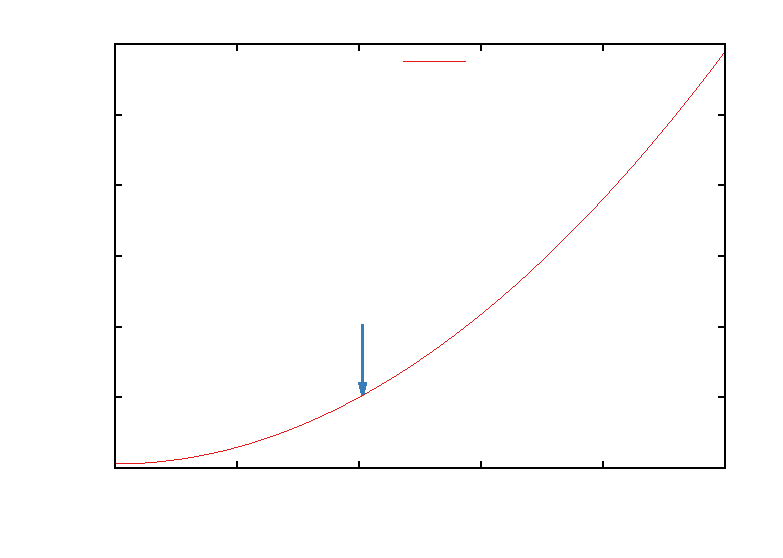
\includegraphics{./plots/abweichung_wellenlaenge}}%
    \gplfronttext
  \end{picture}%
\endgroup

	\caption{Relative Abweichung der Näherungsformel von der exakten Berechnung bei der im Versuch verwendeten Konfiguration: $y_0 = \SI{9.85}{\centi\metre}$, $x_0 = \SI{252}{\centi\metre}$. Der blaue Pfeil markiert die größte vermessene Interferenzordnung $n = 19$.}
	\label{fig:abweichung_wellenlaenge}
\end{figure}

\subsection{Untersuchung der Polarisation des Lasers}

Zur Untersuchung der Polarisation des hier verwendeten Experimentierlasers wird der Intensitätsverlauf an einer Photodiode in Abhängigkeit des Winkels eines davor stehenden Linearpolarisators betrachtet.
Dieser ist in der Lage, einfallendes Licht in eine vorgegebene Richtung linear zu polarisieren.
Für den Fall, dass das einfallende Licht bereits linear polarisiert ist (wie für den hier verwendeten Laser angenommen werden kann), gilt für die hinter dem Polarisator registrierte Intensität (Gesetz von Malus):
\begin{align}
I=I_0\cdot\cos^2\varphi
\end{align}
Der Winkel am Polarisationsfilter wurde in Schritten von \SI{10}{\degree} gedreht und jeweils die Intensität an der Photodiode in \si{\milli\volt} notiert.
In Tabelle \ref{tab:intensitaet} sind die Messwerte festgehalten worden.
\begin{table}
	\centering
	\begin{tabular}{SSSS}
	\toprule
	{Drehwinkel $\varphi / \si{\degree}$} & {Fehler $\Delta\varphi / \si{\degree}$} & {Intensität $I / \si{\milli\volt}$} & {Fehler $\Delta I / \si{\milli\volt}$} \\
	\midrule
	0   & 1 & 39.50 & 0.3 \\
	10  & 1 & 40.00 & 0.3 \\
	20  & 1 & 38.00 & 0.3 \\
	30  & 1 & 33.80 & 0.3 \\
	40  & 1 & 27.90 & 0.3 \\
	50  & 1 & 20.20 & 0.3 \\
	60  & 1 & 13.40 & 0.3 \\
	70  & 1 & 6.45  & 0.3 \\
	80  & 1 & 2.62  & 0.3 \\
	90  & 1 & 0.60  & 0.3 \\
	100 & 1 & 1.10  & 0.3 \\
	110 & 1 & 3.50  & 0.3 \\
	120 & 1 & 8.60  & 0.3 \\
	130 & 1 & 14.70 & 0.3 \\
	140 & 1 & 21.20 & 0.3 \\
	150 & 1 & 27.70 & 0.3 \\
	160 & 1 & 33.40 & 0.3 \\
	170 & 1 & 37.00 & 0.3 \\
	180 & 1 & 38.50 & 0.3 \\
	190 & 1 & 37.50 & 0.3 \\
	200 & 1 & 34.70 & 0.3 \\
	210 & 1 & 29.60 & 0.3 \\
	220 & 1 & 22.90 & 0.3 \\
	230 & 1 & 16.30 & 0.3 \\
	240 & 1 & 9.50  & 0.3 \\
	250 & 1 & 4.10  & 0.3 \\
	260 & 1 & 1.30  & 0.3 \\
	270 & 1 & 0.30  & 0.3 \\
	280 & 1 & 2.00  & 0.3 \\
	290 & 1 & 5.60  & 0.3 \\
	300 & 1 & 10.90 & 0.3 \\
	310 & 1 & 17.60 & 0.3 \\
	320 & 1 & 24.40 & 0.3 \\
	330 & 1 & 30.50 & 0.3 \\
	340 & 1 & 35.60 & 0.3 \\
	350 & 1 & 38.70 & 0.3 \\
	360 & 1 & 39.50 & 0.3 \\
	\bottomrule
\end{tabular}
	\caption{Messwerte der Intensität an der Photodiode in Abhängigkeit des Winkels am Linearpolarisator}
	\label{tab:intensitaet}
\end{table}

\begin{figure}
	\centering
	\begin{tabular}{SSSS}
	\toprule
	{Drehwinkel $\varphi / \si{\degree}$} & {Fehler $\Delta\varphi / \si{\degree}$} & {Intensität $I / \si{\milli\volt}$} & {Fehler $\Delta I / \si{\milli\volt}$} \\
	\midrule
	0   & 1 & 39.50 & 0.3 \\
	10  & 1 & 40.00 & 0.3 \\
	20  & 1 & 38.00 & 0.3 \\
	30  & 1 & 33.80 & 0.3 \\
	40  & 1 & 27.90 & 0.3 \\
	50  & 1 & 20.20 & 0.3 \\
	60  & 1 & 13.40 & 0.3 \\
	70  & 1 & 6.45  & 0.3 \\
	80  & 1 & 2.62  & 0.3 \\
	90  & 1 & 0.60  & 0.3 \\
	100 & 1 & 1.10  & 0.3 \\
	110 & 1 & 3.50  & 0.3 \\
	120 & 1 & 8.60  & 0.3 \\
	130 & 1 & 14.70 & 0.3 \\
	140 & 1 & 21.20 & 0.3 \\
	150 & 1 & 27.70 & 0.3 \\
	160 & 1 & 33.40 & 0.3 \\
	170 & 1 & 37.00 & 0.3 \\
	180 & 1 & 38.50 & 0.3 \\
	190 & 1 & 37.50 & 0.3 \\
	200 & 1 & 34.70 & 0.3 \\
	210 & 1 & 29.60 & 0.3 \\
	220 & 1 & 22.90 & 0.3 \\
	230 & 1 & 16.30 & 0.3 \\
	240 & 1 & 9.50  & 0.3 \\
	250 & 1 & 4.10  & 0.3 \\
	260 & 1 & 1.30  & 0.3 \\
	270 & 1 & 0.30  & 0.3 \\
	280 & 1 & 2.00  & 0.3 \\
	290 & 1 & 5.60  & 0.3 \\
	300 & 1 & 10.90 & 0.3 \\
	310 & 1 & 17.60 & 0.3 \\
	320 & 1 & 24.40 & 0.3 \\
	330 & 1 & 30.50 & 0.3 \\
	340 & 1 & 35.60 & 0.3 \\
	350 & 1 & 38.70 & 0.3 \\
	360 & 1 & 39.50 & 0.3 \\
	\bottomrule
\end{tabular}
	\caption{Anpassung einer zu erwartenden Kurve an die Messwerte}
	\label{fig:malus}
\end{figure}

\subsection{Messung des Strahlprofils und des Stabilitätsgebiets des Lasers}

\subsection{Aufbau der optischen Diode}

\subsection{Optischer Spektrumanalysator}

\subsection{Präzise Messung des Modenabstandes mittels einer optischen Schwebung}

\section{Fazit}


% BIBLIOGRAPHIE
\vspace{\fill}
% Maximale Anzahl der Einträge in Klammer
% Zitieren mit \cite{lamport94}
\begin{thebibliography}{9}
\bibitem{schawlow}
	A. L. Schawlow,
	\emph{Measuring the Wavelength of Light with a Ruler},
	Am. J. Phys., Volume 33, Issue 11 (1965)

\bibitem{NISTSpectra}
	Kramida, A., Ralchenko, Yu., Reader, J., and NIST ASD Team (2014).
	\emph{NIST Atomic Spectra Database} (ver. 5.2).
	\url{http://physics.nist.gov/asd} (Letzter Abruf: 18. Dezember 2014).
	National Institute of Standards and Technology, Gaithersburg, MD.
 
\end{thebibliography}

\clearpage

% APPENDIX
\begin{appendix}
\section{Anhang}


\end{appendix}

\end{document}
